%
%  TODO:
%  - RELIRE POUR LES FOTTES ET ACCENTS
%  - le Q learning
%  -
%

\documentclass{report}
\usepackage{fontspec}
\usepackage{polyglossia}
\usepackage{pgfplots}
\usepackage{tikz}
\usepackage{unicode-math}
\usepackage{amsmath}
\usepackage{listings}
\usepackage{algorithm}
\usepackage{algpseudocode}
\usepackage{subfig}

\usetikzlibrary{patterns,arrows,positioning}

\setmainlanguage{french}

\newcommand{\R}{\mathbb{R}}

\DeclareMathOperator{\card}{card}
\DeclareMathOperator{\argmax}{argmax}
\DeclareMathOperator{\uniform}{Uniform}

\title{Ocaml---IA\\Tetris par Qlearning}
\author{C.~Cousin, G.~Hondet, L.~Pineau, B.~Viry}
\date{\today}

\tikzset{
    %Define standard arrow tip
    >=stealth',
    %Define style for boxes
    punkt/.style={
           rectangle,
           rounded corners,
           draw=black, very thick,
           text width=6.5em,
           minimum height=2em,
           text centered},
    % Define arrow style
    pildwn/.style={
           <-,
           thick,
           shorten <=2pt,
           shorten >=2pt,},
    pilup/.style={
           ->,
           thick,
           shorten <=2pt,
           shorten >=2pt,}
}


\begin{document}
\maketitle
\tableofcontents

\chapter*{Introduction}
\addcontentsline{toc}{chapter}{Introduction}

\chapter*{Notations}
\addcontentsline{toc}{chapter}{Notations}
Seront notées dans la suite du rapport:
\begin{itemize}
  \item \(n_t\) le nombre de tetrominos par jeu,
  \item \(\mathcal{S}\) l'ensemble des états,
  \item \(b_w, b_h\) la largeur et la hauteur totale du plateau.
\end{itemize}
Sauf mention explicite, les applications utiliseront les valeurs \(n_t=10000,
b_w = 6\). Seront distingu\'ees la hauteur totale \(b_h\) et la hauteur relative
à un instant de jeu \(h\) du plateau, la première correspond à la hauteur
théorique maximale atteignable quand la deuxieme concerne la hauteur
effectivement atteinte à un instant de jeu, i.e.\ le nombre de lignes non vides
sur le plateau.

\chapter{Tetris}

\section{Le jeu et sa simplification}
Tetris met le joueur au défi de réaliser des lignes complètes en déplaçant des
pièces de formes différentes, les tétrominos, qui défilent depuis le haut
jusqu'au bas de l'écran. Les lignes complétées disparaissent tout en rapportant
des points et le joueur peut de nouveau remplir les cases libérées. Le jeu
n'a pas de fin: le joueur perd la partie lorsqu'un tétrimino reste bloqué en
haut.

Dans notre version simplifiée, il n'y a pas de limite de hauteur, le jeu se
termine apres avoir fourni 10000 tetrominos à placer. De plus notre
tetris diffère par une grille plus étroite (6 colonnes disponibles), moins de
tetrominos différents (seulement 5) et des tetrominos plus petits (taille
inférieure à 2).

\begin{figure}[h]
  \centering
  \subfloat[Diagonale] {%
    
\begin{tikzpicture}
      \fill[color=magenta] (0,0) rectangle (1,1);
      \fill[color=magenta] (0,0) rectangle (-1,-1);
      \draw (-1,1) rectangle (1,-1);
    \end{tikzpicture}
  }\qquad
  \subfloat[L] {%
    
\begin{tikzpicture}
      \fill[color=cyan] (0,0) rectangle (1,1);
      \fill[color=cyan] (0,0) rectangle (-1,-1);
      \fill[color=cyan] (0,0) rectangle (-1,1);
      \draw (-1,1) rectangle (1,-1);
    \end{tikzpicture}
  }\qquad
  \subfloat[Carré] {%
    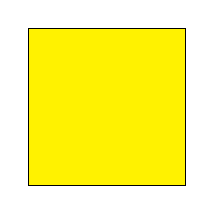
\begin{tikzpicture}
      \fill[color=yellow] (0,0) rectangle (1,1);
      \fill[color=yellow] (0,0) rectangle (-1,-1);
      \fill[color=yellow] (0,0) rectangle (-1,1);
      \fill[color=yellow] (0,0) rectangle (1,-1);
      \draw (-1,1) rectangle (1,-1);
    \end{tikzpicture}
  }\\
  \subfloat[Barre] {%
    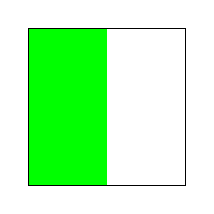
\begin{tikzpicture}
      \fill[color=green] (0,0) rectangle (-1,-1);
      \fill[color=green] (0,0) rectangle (-1,1);
      \draw (-1,1) rectangle (1,-1);
    \end{tikzpicture}
  }\qquad
  \subfloat[Point] {%
    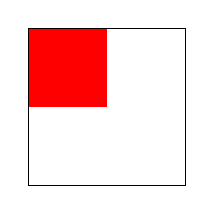
\begin{tikzpicture}
      \fill[color=red] (0,0) rectangle (-1,1);
      \draw (-1,1) rectangle (1,-1);
    \end{tikzpicture}
  }
  \caption{Liste des tertrominos}\label{fig:tetrolist}
\end{figure}

Un tetromino est placé par le choix d'une colonne et d'une orientation.

\section{L'implémentation}

\subsection{Représentation}

\paragraph{Tetrominos}
Les tetrominos sont tableaux de longueur 4. L'unidimensionnalité permet
d'implémenter les rotations comme des transformations d'indices, évitant la
création ou la modification de structures.

Les tetrominos sont tous de même dimension par souci d'homogénéite.

\paragraph{Plateau \texttt{Board}}
Le plateau est représenté par une matrice de dimension
\(2\cdot n_t \times 6\) d'entiers dans laquelle on inscrit les tetrominos. Les
manipulations du plateau se font en place.


\paragraph{Actions}
Composées d'une rotation et d'une translation. Elles permettent d'agir sur les
tetrominos. Les rotations sont representées par les points cardinaux
(North, South, East, West) et les translations par un entier compris entre 0 et
\(b_w - 2\) correspondant à l'indice du coin supérieur gauche du tetromino
(voir fig\ref{fig:tetref}).

\begin{figure}[h]
  \centering
  \subfloat[Diagonale] {%
    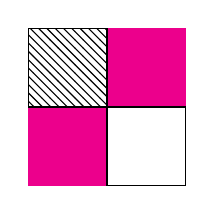
\begin{tikzpicture}
      \fill[color=magenta] (0,0) rectangle (1,1);
      \fill[color=magenta] (0,0) rectangle (-1,-1);
      \draw[pattern = north west lines] (0,0) rectangle (-1,1);
      \draw (0,0) rectangle (1,-1);
    \end{tikzpicture}
  }\qquad
  \subfloat[L] {%
    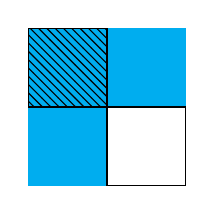
\begin{tikzpicture}
      \fill[color=cyan] (0,0) rectangle (1,1);
      \fill[color=cyan] (0,0) rectangle (-1,-1);
      \fill[color=cyan] (0,0) rectangle (-1,1);
      \draw[pattern = north west lines] (0,0) rectangle (-1,1);
      \draw (0,0) rectangle (1,-1);
    \end{tikzpicture}
  }
  \caption{Point de reference de tetromino, ici hachure}\label{fig:tetref}
\end{figure}

La geometrie de certains tetrominos rend certaines orientations redondantes. Par
exemple le carre est invariant par rotation, et utiliser les quatre rotations
ne fait qu'augmenter inutilement le nombre d'actions possibles, et augmente par
consequent la quantite d'information que l'agent doit apprendre. Pour pallier
cette redondance, chaque tetromino dispose de son propre ensemble de rotations
applicables.

\section{Déroulement d'une partie}
Un tetromino choisi aleatoirement parmi les cinq disponibles est donne au
joueur. Ce dernier doit alors choisir ou et comment le placer. Une fois ce
choix effectue, le tetromino est place en respectant les contraintes du jeu. Le
plateau est ensuite mis a jour: les lignes completes sont supprimees et la
hauteur est reevaluee. Un nouveau tetromino est donne et le jeu continue.


Lors d'une partie le joueur doit poser les pièces qui lui sont proposées sur
le plateau de jeu. Il est donc nécessaire d'utiliser une fonction \texttt{play}
qui permet de placer une pièce sur le plateau. La pièce ``tombe'' donc dans la
colonne sélectionnée tant qu'elle ne rencontre pas d'obstacle (fond du plateau
ou un autre tétromino). Pour cela, il y a besoin d'une fonction de test de
collision, qui renvoie si l'emplacement testé peut accueillir le tetromino.
S'il y a collision, on sélectionne le dernier emplacement libre et on place la
pièce.

Lorsqu'une ligne est entièrement remplie, elle est supprimée du tableau, mais
la taille totale du plateau reste la même.

\section{Drawbacks}
\subsection{Fonction collide}
L'implémentation actuelle oblige l'accessibilité de la position finale depuis
le haut du plateau car la pièce ne peut pas être glissée au dernier moment
sous une autre.
\subsection{Tetromino}
Les tetrominos sont tous de même dimension par souci d'homogénéite et cela
peut entrainer un probleme de ``tetromino flottant''. Ce problème est traité par
un choix d'action spécifique à chaque pièce (cf ~\ref{sec:volant}).


\chapter{Q learning}

\section{principe de l'apprentissage par renforcement et Q-learning}
\subsection{L'apprentissage par renforcement, késako ?}

L'apprentisage par renforcement est une méthode d'apprentisage automatique
inspirée de la biologie. L'idée est un apprentisage à partir d'actions et
de récompenses, à l'image d'un enfant qui met les doigts dans une prise, il
risque d'apprendre et ne plus recommencer.

Un agent est plongé dans un environnement (ici le jeu de Tetris) et effectue une
action (pour nous un mouvement). L'agent reçoit alors une récompense (ou alors
une punition) qui lui permet d'adapter son comportement et ainsi apprendre à
évoluer dans l'environnement.

\begin{figure}[h]
    \begin{center}
        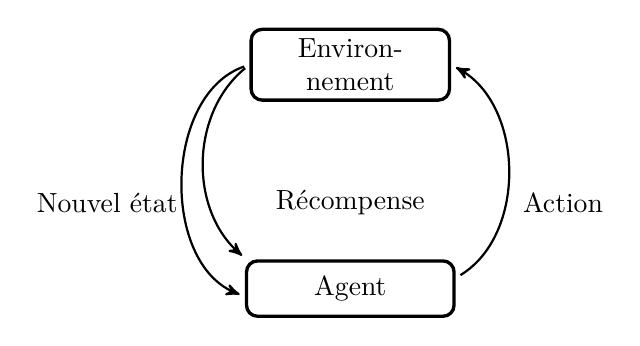
\begin{tikzpicture}[node distance=1cm, auto,]
         %nodes
         \node[punkt] (env) {Environnement};
         \node[punkt, inner sep=5pt,below=2cm of env]
         (agent) {Agent}
            edge[pilup,bend right=60] (env.east)
            edge[pildwn,bend left=70] (env.west)
            edge[pildwn,bend left=50] (env.west);
        \node[left=of env,below=of env] (rew) {Récompense};
        \node[left=of rew] {Nouvel état};
        \node[right=of rew] {Action};
        \end{tikzpicture}
    \end{center}

    \caption{Principe d'apprentissage par renforcement}
    \label{}
\end{figure}

Le but de l'apprentissage va être de maximiser la somme des récompense sur une
période donnée.

Plus formellement, notons:
\begin{itemize}
    \item \( s_i \) un état à l'étape \( i \)
    \item \( a_i \) une action jouée à l'étape \( i \)
    \item \( r(s_i, a_i) \) la récompense immédiate après l'action \( a_i \)
    \item \( \gamma \) la vision de l'agent (cf.~\ref{sec:algorithmes}).
\end{itemize}

La récompense à long terme pour un ensemble
\( s = (s_0, a_0, s_1, a_1, \hdots) \) est donc:
\[
  R(s) = \sum_{i=0}^{+\infty}\gamma^i \cdot r(s_i, a_i)
\]


\subsection{Le Q-learning}



\section{Représentation des états}

\subsection{Composition}
Intuitivement, un état correspond à la pièce donnée à jouer et la disposition
des pièces sur le plateau, ce qui correspond aux informations nécessaires pour
le placement d'une pièce par l'agent. En notant \(n_t\) le nombre de tetrominos
différents, \( h \) la hauteur du plateau a un instant considèré  et \(w\) la
largeur du plateau, on obtient \(n_t \cdot 2^{h \cdot b_w}\) états possibles.

Pour réduire le nombre d'états, on ne considère que les deux plus hautes lignes
contenant au moins un tetromino. On obtient \(5\cdot 2^{2 b_w}\) états
possibles, soit \(20480\) pour une largeur \( b_w = 6 \).

\subsection{Codage}
Comme chaque état correspond \textit{in fine} à une ligne de la matrice Q, il est
nécessaire d'avoir une bijection entre l'ensemble des états et les entiers. La
bijection genère deux représentations entières, une pour les deux lignes de
l'état et l'autre pour la pièce, et les combine en un état entier final,
\[
  \texttt{get\_state}\colon [0,4]\times [0, 2^{12} - 1] \to [0, 5\cdot 2^{12}].
\]


\section{Algorithmes}\label{sec:algorithmes}

L'algorithme~\ref{alg:action} concerne la maniere dont l'agent choisit les
actions parmi l'ensemble des actions possibles \(\mathcal{A}\), etant donne un
etat \(s\). Le parametre \(\epsilon\) definit la frequence de choix aleatoire.
\begin{algorithm}
  \caption{Choix de l'action}\label{alg:action}
  \begin{algorithmic}
    [1]
    \Procedure{ChooseAction}{$Q$, $s$, $\mathcal{A}$}
    \State{} tirage \(\gets \uniform([0, 1])\)
    \If{tirage \(> \epsilon\)}
    \Return{\(\argmax_{a\in\mathcal{A}} Q(s, a)\)}\Comment{Choix de l'action
    maximisant l'esperance de recompense}
    \Else{}
    \Return{\(\uniform(\mathcal{A})\)}\Comment{Choix aleatoire}
    \EndIf{}
    \EndProcedure{}
  \end{algorithmic}
\end{algorithm}


L'algorithme~\ref{alg:qlearning} definit la maniere dont l'agent se met a jour
afin de maximiser l'esperance de gain. Est notee \(\gamma\) la vision de
l'agent correspondant a l'importance que l'agent attribue aux recompenses
futures par rapport a la recompense immediate. Un \(\gamma\) de zero cree un
agent myope ne choisissant son action que par rapport a la recompense immediate
tandis qu'un \(\gamma\) tendant vers un associe autant d'importance aux
recompenses des coups suivants qu'a la recompense immediate.
\begin{algorithm}
  \caption{Algorithme de \textit{Q-learning}}\label{alg:qlearning}
  \begin{algorithmic}
    [1]
    \Procedure{Update}{$Q$, $\epsilon$, $\gamma$, $\alpha$}
    \Repeat{}
    \State{} initialisation de \(s\)
    \Repeat{}
    \State{} \(a \gets\) ChooseAction$(Q, s, \mathcal{A}, \epsilon)$
    \State{} jouer \(a\), observer \(r\) et le nouvel \'etat \(s'\),
    \State{} \(Q(s, a) \gets Q(s, a) + \alpha\left[ r + \gamma \max_{a'}
      Q(s', a') - Q(s, a)\right]\)
    \Until{$s$ est terminal}
    \Until{entrainement fini}
    \EndProcedure{}
  \end{algorithmic}
\end{algorithm}

Pour realiser une mise a jour, l'agent commence par choisir l'action qui, a un
etat donne fournit l'esperance de recompense maximale, selon les connaissances
actuelles de l'agent. Une fois le coup joue, l'agent recoit une recompense
evaluant evaluant l'impact du coup choisi sur l'environnement. L'agent utilise
cette recompense et sa connaissance des etats resultants pour affiner
l'esperance de recompense associee au coup qu'il vient de realiser.

\subsection{Paramètres}
L'apprentissage est paramétré par les trois variables,
\begin{itemize}
  \item \(\alpha \in [0, 1]\) le taux d'apprentissage,
  \item \(\epsilon \in [0, 1]\) la fréquence de coups aléatoires effectués,
  \item \(\gamma \in [0, 1]\) la vision de l'agent.
\end{itemize}
Pour assurer la convergence de la matrice vers la matrice optimale,
le taux d'apprentissage doit évoluer au cours des entrainements.
D'après~\cite{watkins92}, la suite \( (\alpha_k)_k \) doit vérifier
\( \sum_{k=0}^\infty \alpha_k = \infty \) et \(
\sum_{k=0}^\infty \alpha_k^2 \in \R \). La suite choisie a donc la forme
suivante, pour tout \( k \in \mathbb{N} \) et
\( C \in \R \backslash \{ \frac{-1}{k} \} \):
\[
  \alpha_k = \frac{1}{1 + Ck}.
\]
Le taux d'apprentissage reste manipulable via le paramètre \( C \).


% Le paramètre \(\epsilon\) pourra \'egalement varier au cours des jeux effectués.
% En effet, intuitivement, un \(\epsilon\) grand permet une exploration rapide de
% l'ensemble des états possibles mais devient nuisible lorsque la matrice est bien
% entrainée.

Le paramètre \(\epsilon\) répond au problème exploration contre exploitation. En
effet, un \(\epsilon\) important permet une exploration rapide de l'ensemble
des états possibles en jouant des actions aléatoires. À l'inverse un \(\epsilon\)
petit correspond à l'exploitation de la politique apprise par l'agent. Ainsi,
une diminution d'\(\epsilon\) au cours de la phase d'apprentissage permet de
stabiliser les resultats obtenus.

\begin{figure}
  \centering
  \begin{tikzpicture}
    \begin{axis}[line width=0.05, mark size = 0.1,
        legend entries={0,.0003,.0006,.0009}
      ]
      \foreach \i in {0,1,...,3}{%
        \addplot+ table [x expr = {\lineno}, y index = \i] {data/epsilon.dat};
      }
    \end{axis}
  \end{tikzpicture}
  \caption{Exploitation ou exploration?}
\end{figure}

\paragraph{Valeurs}
\begin{figure}
  \centering
  \begin{tikzpicture}
    \begin{axis}[line width=0.05, mark size = 0.1,
        legend entries={0.80,0.84,0.88,0.92,0.96,1.00}
      ]
      \foreach \i in {0,1,...,5}{%
        \addplot+ table [x expr = {\lineno}, y index = \i] {data/gamma.dat};
      }
    \end{axis}
  \end{tikzpicture}
  \caption{Influence du parametre \(\gamma\)}
\end{figure}



\chapter{Minimisation d'une fonction objectif \( V \)}

\section{Représentation des états et transitions}

Dans cette partie l'ensemble des états \( \mathcal{S} \) est égal à l'ensemble
des plateaux possibles. \( s \in \mathcal{S} \) est un plateau particulier.

\section{Nouvelle méthode d'apprentissage}

Pour s'affranchir de la limite de memoire due au nombre d'etats possibles, la
matrice est remplacee par une fonction objectif \( V \) tel que:
\[
\forall s \in \mathcal{S}, \qquad V(s) =
\mathbb{E}(\sum_{t=0}^{+\infty} \gamma ^t \cdot r_t)
\]
qui estime l'espérance de gain à partir d'un plateau donné.
L'apprentissage consiste donc maintenant à la maximisation de la
fonction \( V \).
On suppose \( V \) linéaire \(V \colon \R^n \to \R\). Cette fonction est alors
déterminée par un ensemble de poids \(w = (w_0\, w_1\, \dots\, w_n)^\top\)
qu'il va falloir 'entrainer'.

En notant \( s_t \) un plateau de jeu à un instant \( t \), et
\(\phi_i\colon \mathcal{S} \to \R\) des caracteristiques du plateau
(voir~\cite{boumaza13}), la fonction \(V\)
est définie par:
\[
  V \colon s_t \mapsto w_0 + \sum_{i=1}^n w_i \cdot \phi_i (s_t)
\]

On appelle transition un tuple \( (s_t, a_t, r_t, s_{t+1}) \), Avec:
\begin{itemize}
    \item \( s_t \) le plateau à l'étape \( t \)
    \item \( a_t \) l'action joué à l'étape \( t \)
    \item \( r_t \) la récompense joué à l'étape \( t \)
    \item \( s_{t+1} \) le plateau résultant de l'action \( a_t \)
\end{itemize}


\section{Algorithme}

L'algorithme d'apprentissage utilisé dans cette partie repose sur une variante
sochastique de l'algorithme par descente de gradient.

L'idée est de jouer \( B \) coups et enregistrer dans une mémoire les différentes
transitions. Les coups sont choisis selon l'algorithme~\ref{alg:choseactionv2}.

\begin{algorithm}[h]
  \caption{Choix de l'action}\label{alg:choseactionv2}
  \begin{algorithmic}
    [1]
    \Procedure{ChooseAction2}{$V$, $s_t$, $\mathcal{A}$}
    \State{} tirage \(\gets \uniform([0, 1])\)
    \If{tirage \(> \epsilon\)}
    \State{}\Return{\(\argmax_{{a_t}\in\mathcal{A}} [r_t + \gamma V(s_{t+1})] \)}
    \\ \Comment{Choix de l'action maximisant l'esperance de recompense}
    \Else{}
    \State{}\Return{\(\uniform(\mathcal{A})\)}\Comment{Choix aleatoire}
    \EndIf{}
    \EndProcedure{}
  \end{algorithmic}
\end{algorithm}

Pour ne pas sauvegarder plusieurs fois le plateau de jeu \(s_t\), on ne met en
mémoire que les features intéressantes \( (\phi_1 (s_t), \hdots, \phi_7(s_t)) \).

Une fois la mémoire \( \mathcal{M} \) remplie avec \( B \) transitions, on calcule \( \delta_t \):
\[
\forall t_t = (s_t, a_t, r_t, s_{t+1}) \in \mathcal{M},\quad
\delta(t_t) = \underbrace{r_t + \gamma \cdot V(s_{t+1})}_{target} -
\underbrace{V(s_{t})}_{prediction}
\]
Comme \( V \) estime l'espérance de gain, un agent bien entrainé doit annuler
les différents \(delta_t\) (l'espérance prédite à l'instant t = la récompense
à l'instant t + l'espérance prédite à l'instant t + 1).

On définit alors une fonction de coup (loss function):
\[
\mathcal{L} = \frac{1}{2B} \sum _{t_t \in \mathcal{M}} \delta(t_t)^2
\]

On applique alors l'algorithme de descente de gradient pour minimiser la fonction
\( \mathcal{L} \) en actualisant les poids \( w \) suivant:
\[
w = w - \eta \nabla \mathcal{L}
\]

La procédure est synthétisé dans l'algorithme suivant:

\begin{algorithm}[H]
  \caption{Algorithme d'apprentissage d'une fonction lineaire}\label{alg:linfct}
  \begin{algorithmic}
    [1]
    \Procedure{Update}{$V$, $\epsilon$, $\gamma$, $\eta$, $\eta$}
    \Repeat{}
    \State{} initialisation de \(s\)
    \Repeat{}
    \For{1 to $B$}
    \State{} \(a \gets \mathup{ChooseAction2}(V, s, \mathcal{A}, \epsilon)\)
    \State{} joue \(a\), observer \(r\) et le nouvel \'etat \(s'\)
    \State{} ajouter a la memoire \( \left(\phi(s), a, r, \phi(s')\right) \)
    \EndFor{}
    \State{} Chosir aleatoirement \(B\) quadruplets depuis la memoire
    \State{} \(y_t \gets r_t + \gamma V\left(\phi(s_t')\right)\)
    \State{} \(\delta_t \gets y_t - V \left(\phi(s_t)\right)\)
    \State{} \(\mathcal{L} \gets \frac{1}{2B}\sum_{k=1}^B \delta_t^2\)
    \State{} \(w \gets w - \eta \nabla_w \mathcal{L}\)
    \Until{$s$ est terminal}
    \Until{Entrainement fini}
    \EndProcedure{}
  \end{algorithmic}
\end{algorithm}

\chapter{Difficultés rencontrées}

\section{Le fl\'eau de la mutabilité}
L'usage du \texttt{Array.blit} s'est revélé plus delicat que prévu. En
considerant que la ligne \(l\) doit etre supprimée et en notant \(h\) la hauteur
actuelle du plateau, le principe est de copier la section de tableau incluant
les lignes \(l+1\) jusqu'à \(h+1\) une ligne en dessous, i.e.\ translater le
bloc d'une ligne vers le bas.

Cette démarche engendre des comportements anormaux car la ligne \(h+1\) n'est
pas copiée sur la ligne \(h\), elles partagent la même adresse mémoire. Ainsi,
il etait observé quelques coups après un blit un dédoublement de carrés de
tetrominos, faisant augmenter la hauteur.

Pour pallier ce problème de partage d'adresse mémoire, la ligne \(h\) est
recréée à chaque blit.

\section{Le hollandais volant}\label{volant}
La fonction collide permet de tester la collision du tetromino avec les autres
pièces et le fond du plateau. Lors de l'éxécution de la fonction \texttt{play}
on testait donc toutes les positions possibles pour déposer les pièces de
dimension 2 \(\times \) 2 sur le fond du plateau s'il n'y avait pas eu de
collision. Malheureusement, certaines pièces comme le point ou la ligne
pouvaient avoir une ``ligne vide'' en bas sous certaines rotations. Pour
résoudre ce problème qui est devenu évident après la résolution du problème de
\texttt{Array.blit}, nous avons décidé de restreindre les états possibles dans
la Q-matrice. En effet lors de l'initialisation de la Q-matrice, tous les états
accessibles sont mis à 0 (flottant) et tous les états non utilisés sont
initialisés à \(-\infty \). Ainsi, pour le point, on ne gardera que les
rotations \texttt{South} et \texttt{West}.

\section{Le foncteur n'est pas pass\'e}
Ayant deux moyens pour r\'esoudre le tetris, il semble pertinent de
g\'en\'eraliser le code afin de faire en sorte que toute impl\'ementation
d'agent soit facilement d\'eveloppable et int\'egrable au reste du projet. Pour
cela un foncteur est indiqu\'e: ce foncteur \texttt{Agent.Make} prendrait en
param\`etre un module d'impl\'ementation d'agent, contenant une fonction
permettant de choisir une action, un fonction de mise \`a jour de l'agent, un
type d\'esignant la donn\'ee avec laquelle travaille l'agent (e.g.\ matrice de
flottants pour le Q learning et tableau de poids flottants pour la fonction de
valuation). Le r\'esultat de l'application de ce foncteur est un module ayant
une fonction \texttt{train} entra\^inant en place l'agent, une fonction
\texttt{play} pour jouer un jeu de tetris et une fonction make pour cr\'eer un
agent inital.

La g\'en\'eralisation du code s'est malheureusement r\'ev\'el\'ee plus
d\'elicate que pr\'evu. D'une part les deux m\'ethodes impl\'ement\'ees
contenaient des diff\'erences, notamment sur le nombre de param\`etres, ou
l'utilisation d'une m\'emoire, d'autre part adapter le code \`a ces deux
impl\'ementations finissait plus \`a resembler \`a du bricolage plut\^ot qu'\`a
de la g\'en\'eralisation. Et de plus cela avait tendance \'a pervertir le code
d\'evelopp\'e pour la fonction de valuation, le poussant \`a coller \'a la
signature d'un argument de foncteur qui est peut-\^etre mal designed.

En cons\'equence, l'agent utilisant la fonction d'\'evaluation est cod\'e sur
une branche d\'edi\'ee du git, la branche \texttt{valuation}. Le code du
foncteur est disponible sur la branche \texttt{functorise}.
\chapter{Réesultats du projet}

\chapter*{Conclusion}
\addcontentsline{toc}{chapter}{Conclusion}

\begin{thebibliography}{9}
    \bibitem{watkins92}
    Christopher~J.C.H.~Watkins, Peter~Dayan,
    \textit{Q-Learning, Machine Learning}
    1992.
    \bibitem{deepmind}
    Voloddymyr~Mnih, Koray Kavukcuoghlu, David Silver, Alex Graves, Ioannis
    Antonoglou, Daan Wierstra, Martin Riedmiller,
    \textit{Playing Atari with Deep Reinforcement Learning}
    \bibitem{boumaza13}
    Amine Boumaza,
    \textit{How to design good Tetris players}
    2013.
\end{thebibliography}

\end{document}
